\section{System Architecture and Microservices Design}

\subsection{Architectural Paradigm and Operational SLAs}
To satisfy the demanding throughput, low-latency requirements, and strict analytical security boundaries of enterprise e-commerce, HUB is architected around a decentralized \textbf{Four-Tier System Architecture}. The architecture decouples interactive transaction processing from heavy batch machine learning workloads, enforcing strict service-level agreements (SLAs):
\begin{itemize}
    \item \textbf{Recommendation Serving SLA:} 95th-percentile (P95) response latency under $65\,\text{ms}$ for Top-12 personalized candidate inference.
    \item \textbf{Role-Based Isolation (RBAC):} Cryptographic isolation preventing unauthorized cross-role resource modification using stateless JSON Web Tokens (JWT).
    \item \textbf{Fault Resilience:} Autonomous fallback to national bestselling heuristics in the unlikely event of model inference or feature lookup failures.
\end{itemize}

\begin{figure}[H]
    \centering
    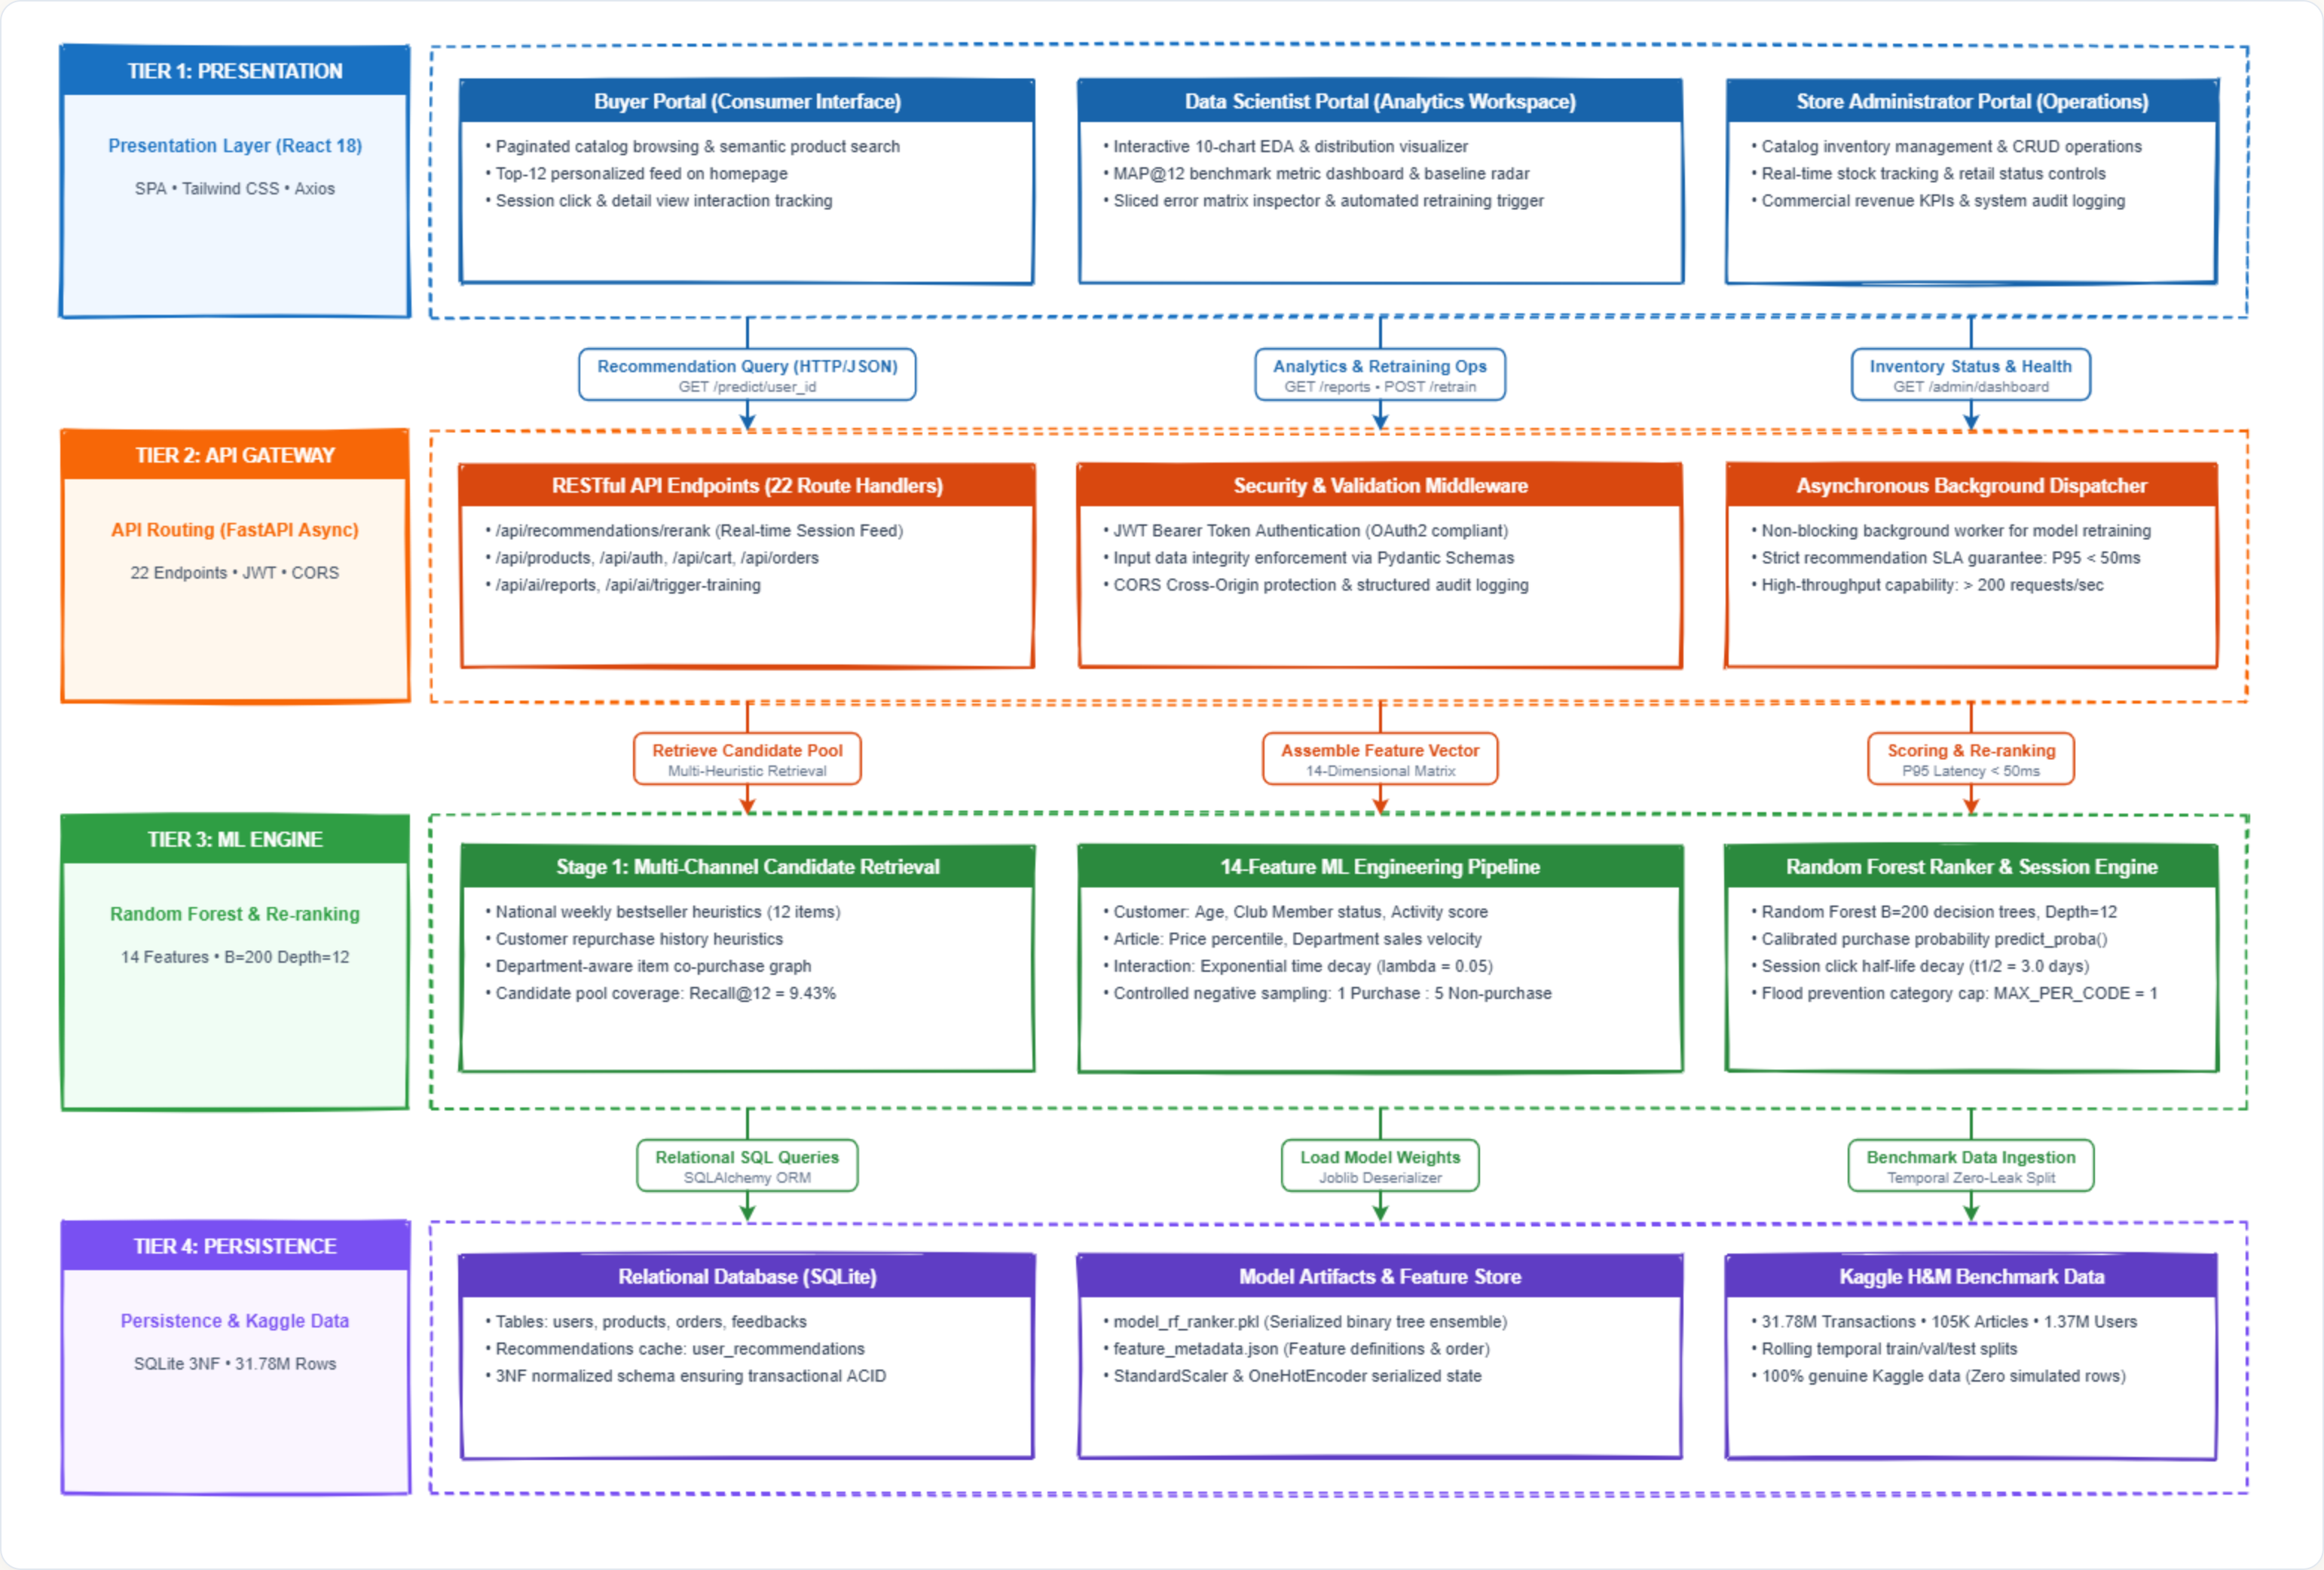
\includegraphics[width=0.95\textwidth]{excalidraw_01_architecture_4tier.png}
    \caption{Four-Tier Decentralized System Architecture of the HUB Recommendation Platform}
    \label{fig:architecture_4tier}
\end{figure}

\subsection{Decomposition of the Four-Tier Model}

\subsubsection{Tier 1: Presentation Layer (React 18 SPA + Vite)}
The client surface is implemented as a modern Single-Page Application (SPA) leveraging React 18, TypeScript, and TailwindCSS. It provides three role-customized viewports:
\begin{itemize}
    \item \textit{Buyer Portal:} Fluid catalogue navigation, real-time search auto-completion, animated cart slide-over drawer, responsive product cards, and instant visual re-ranking updates upon user clicks.
    \item \textit{Data Science Studio:} Interactive EDA chart grids, model performance radar canvases, sliced error matrix diagnostics, and MLOps retraining consoles.
    \item \textit{Admin Control Center:} Tabular interfaces for user privilege management, catalogue stock adjustment, and order status transitions.
\end{itemize}

\subsubsection{Tier 2: Application \& Inference Gateway (FastAPI Gateway)}
The middle tier utilizes Python's asynchronous \textbf{FastAPI} runtime powered by Starlette and Pydantic validation. The application tier exposes RESTful JSON endpoints grouped into modular domain routers:
\begin{enumerate}[(a)]
    \item \texttt{/auth}: OAuth2-compatible token issuance, credential hashing with bcrypt, and RBAC authorization decorators.
    \item \texttt{/products}: High-performance paginated queries with multi-faceted filtering across 5 index groups and 11 garment categories.
    \item \texttt{/recommendations}: Serves precomputed Top-12 ranking lists augmented on-the-fly by the real-time session decay re-ranking engine.
    \item \texttt{/data-science}: Exposes pipeline execution logs, training configuration persistence, and model degradation resolution triggers.
\end{enumerate}

\subsubsection{Tier 3: Persistence Layer (Relational Storage \& Caching)}
Relational persistence is abstracted through SQLAlchemy ORM, supporting both SQLite for localized development and PostgreSQL for scalable production deployments. The relational schema is structured into third normal form (3NF):
\begin{itemize}
    \item \texttt{users}: Authentication credentials, hashed passwords, and assigned role IDs ($2=\text{Buyer}$, $3=\text{Admin}$, $4=\text{Data Scientist}$).
    \item \texttt{products}: Master article records, department hierarchies, pricing percentiles, and stock counters.
    \item \texttt{orders} and \texttt{order\_items}: Immutable transaction ledger recording customer purchases and shipping metadata.
    \item \texttt{user\_interactions}: Fine-grained event streaming capturing real-time click, cart, and wishlist timestamps for in-session re-ranking.
    \item \texttt{user\_recommendations}: Pre-scored Top-12 recommendation tuples serialized from nightly batch training runs.
\end{itemize}

\subsubsection{Tier 4: Model Artifact Tier (Kaggle Cloud Engine \& Storage)}
Heavy machine learning retraining tasks are offloaded to Kaggle Cloud Kernels (4-core vCPU, 30GB RAM). Serialized models (\texttt{model\_rf\_ranker.pkl}), feature scalers (\texttt{scaler.pkl}), and evaluation summaries are versioned under timestamped directory runs (\texttt{data\_scientist/runs/<run\_id>/}) before atomic synchronization into production tables.

\subsection{System Use-Case Modeling}
The functional capabilities of the system across the three primary actors are modeled in the comprehensive Use-Case diagram shown in Figure \ref{fig:usecase_diagram}.

\begin{figure}[H]
    \centering
    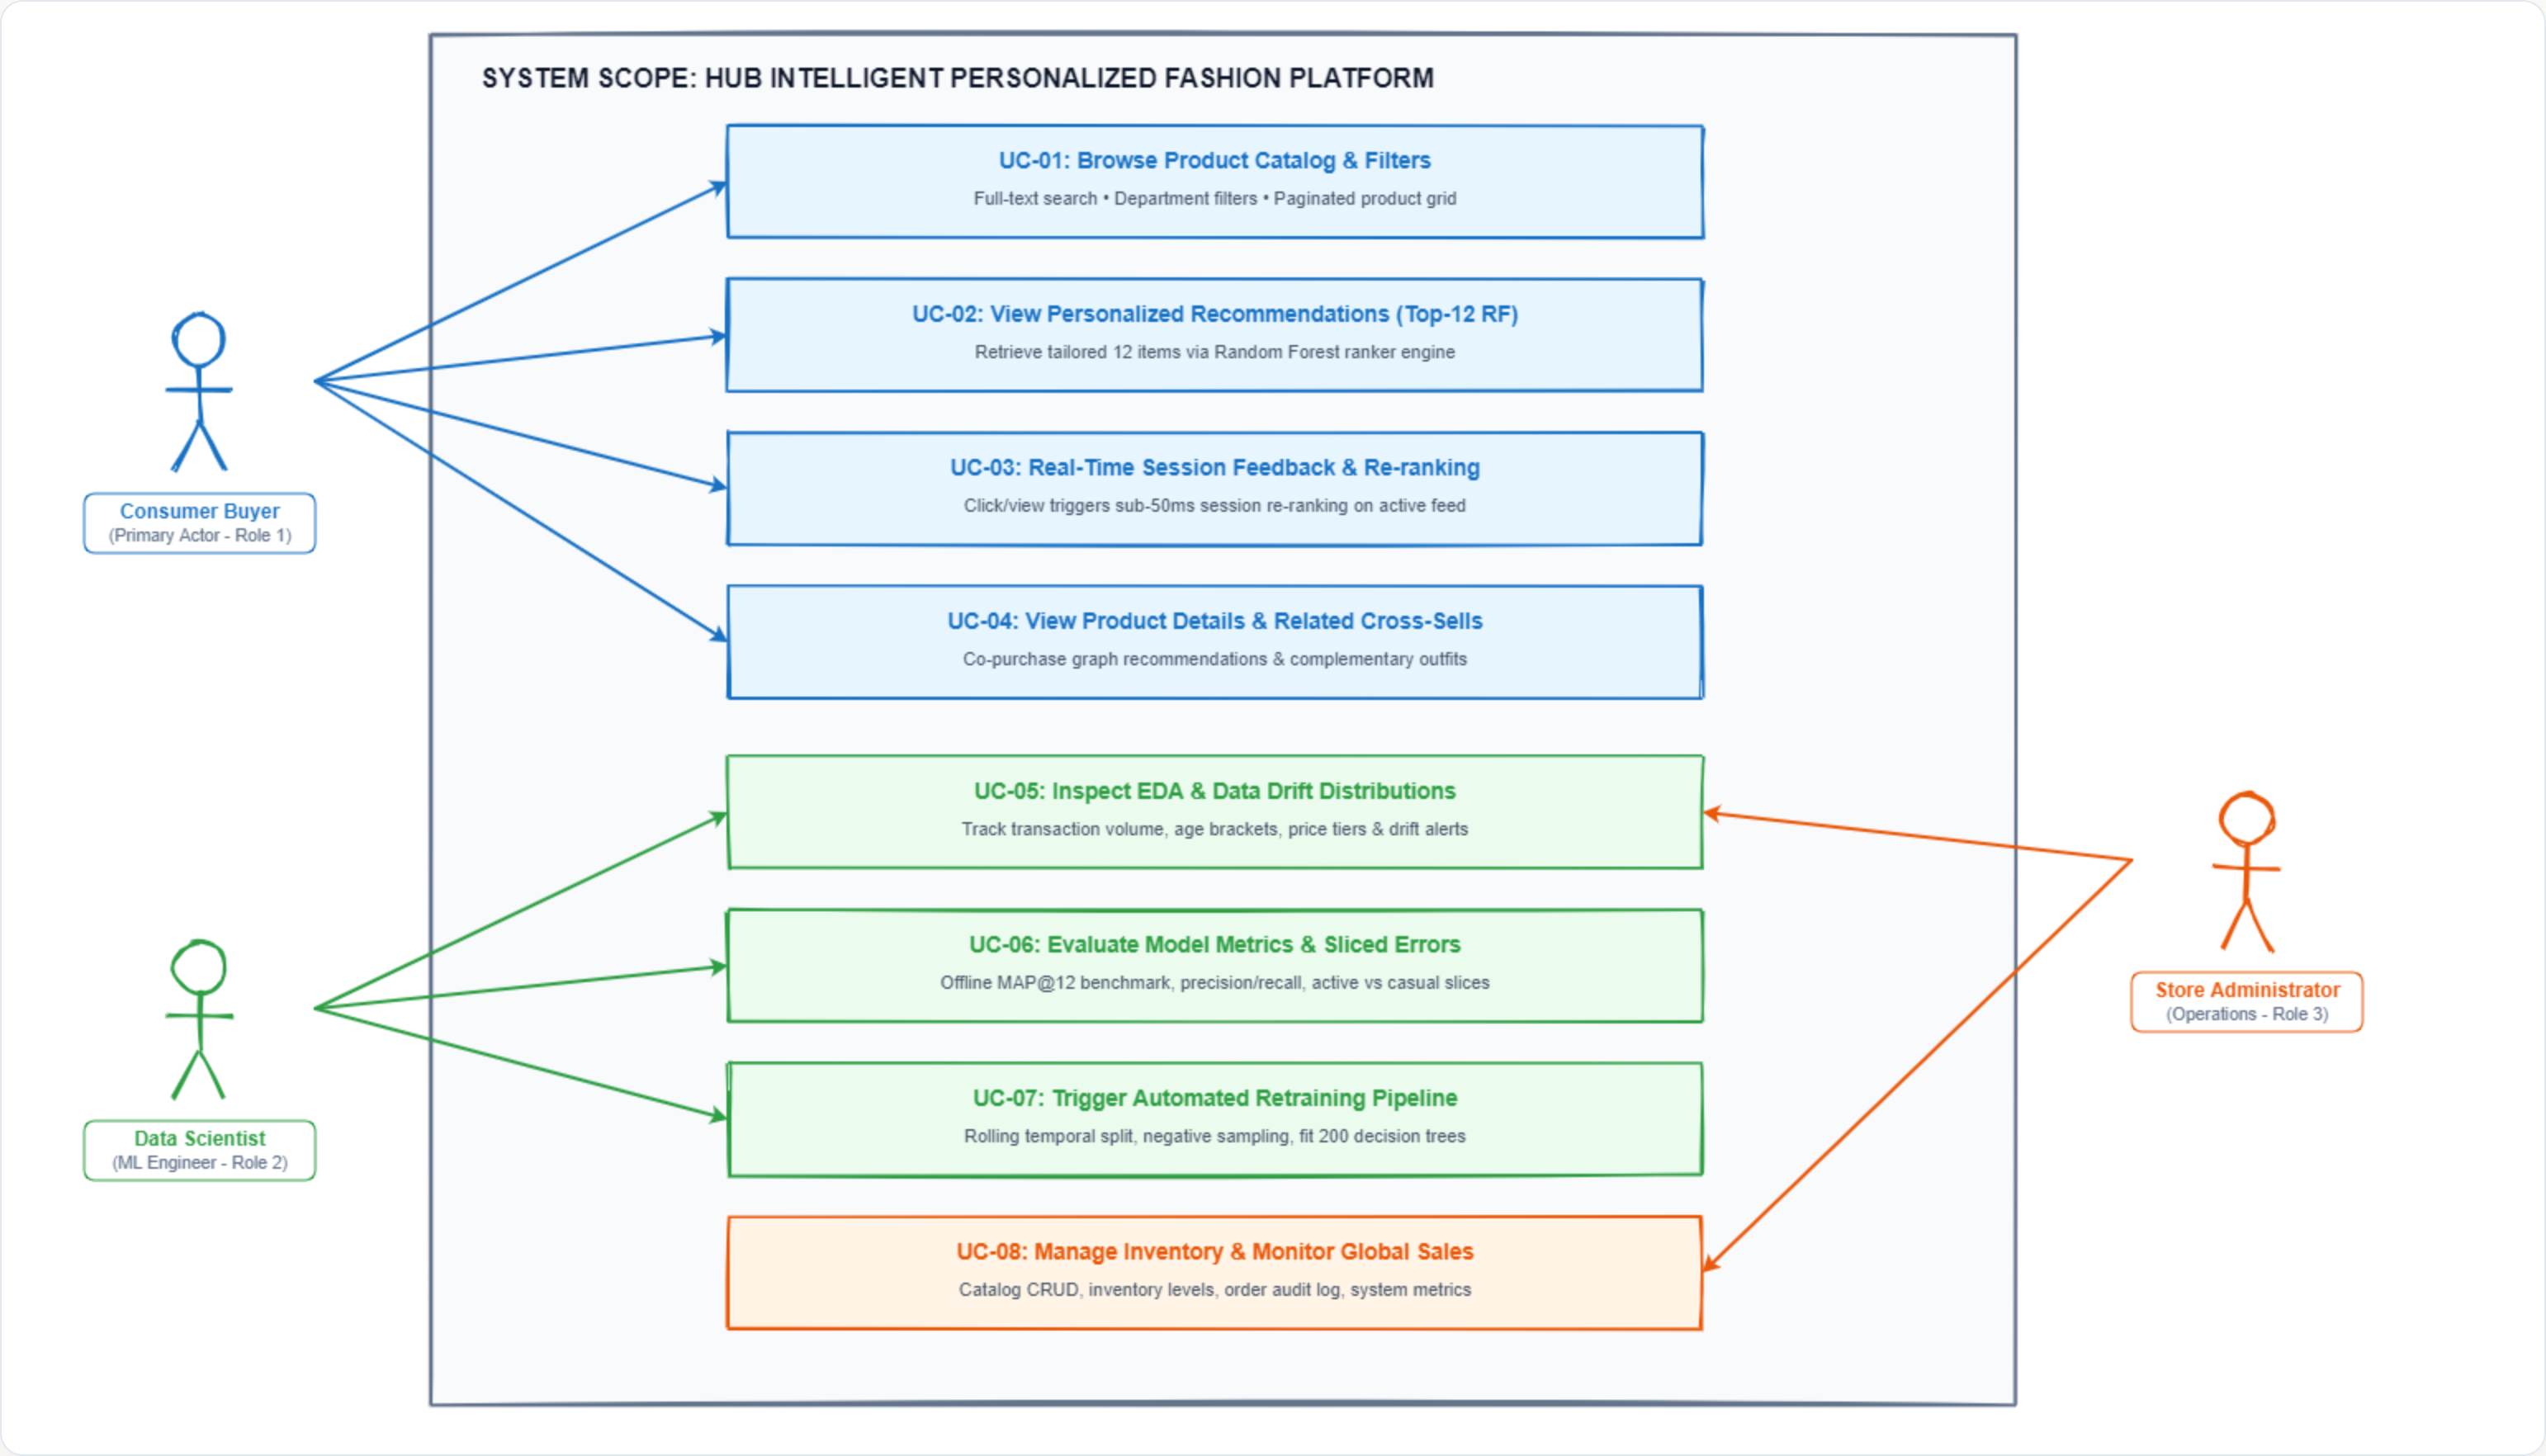
\includegraphics[width=0.95\textwidth]{excalidraw_02_usecase_diagram.png}
    \caption{UML Use-Case Specification Diagram Across Buyer, Data Scientist, and Administrator Roles}
    \label{fig:usecase_diagram}
\end{figure}
